\section{Data Collection}

\subsection{Pre-processing}


In summary, we extract the following fields from each patent that we parse:

\begin{itemize}
\item {Attributes for co-inventorship graph}:
Inventor name, inventor address, assignee name, assignee address, year of patent grant.

\item {Attributes for citation graph}:
Patent ID, name and address of all the inventors and assignees, year of patent grant, all the patents who cites this patent.
\end{itemize}



\subsection{Author \& Organisation Disambiguation}


Figure~\ref{process} summarises the data collection, parsing and clensing phases we employ in our 

\begin{figure}[H]
		  \centering	
          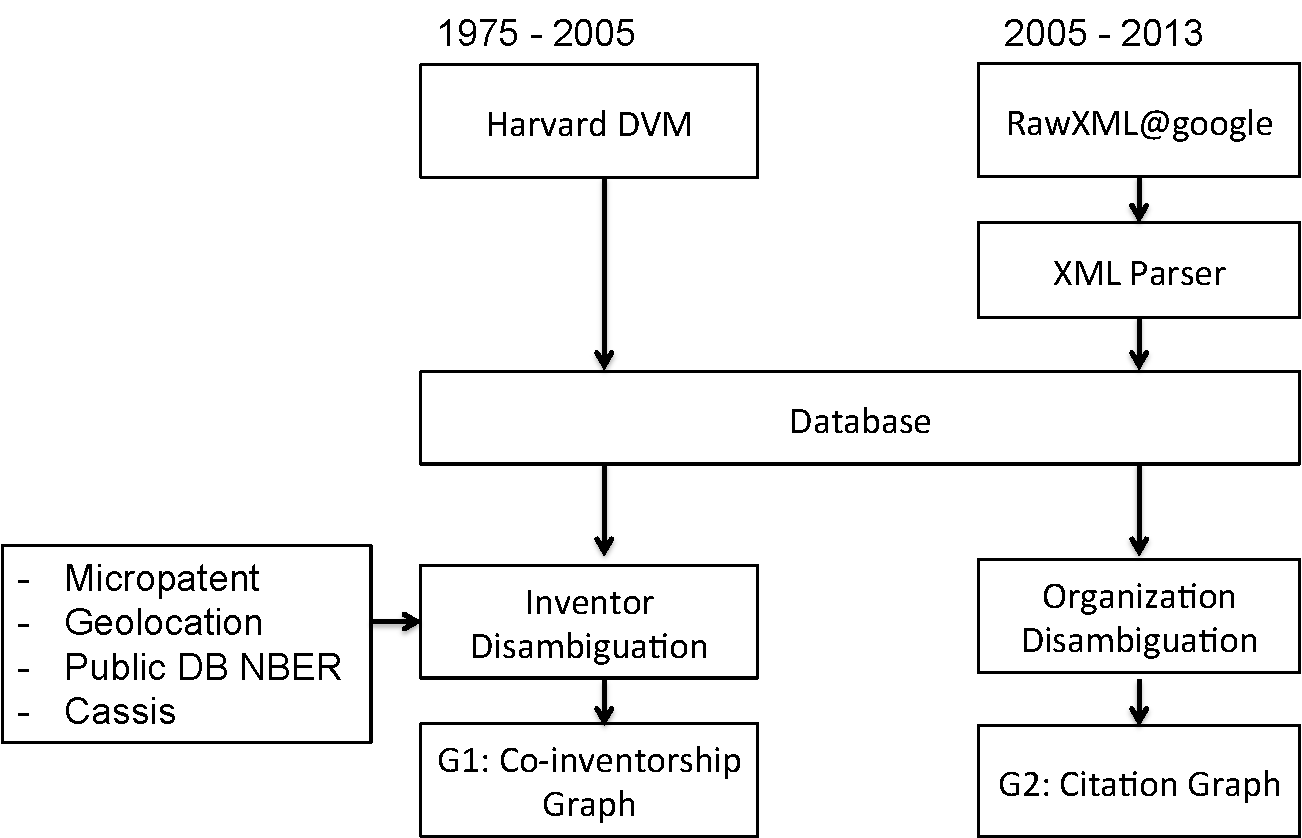
\includegraphics[scale=0.6]{../figures/process.pdf}
          \label{process}
          \caption{Overview of data collection and pre-processing steps to generate the co-inventorship and citation graphs for this study.}
\end{figure}


\subsection{Graph Construction}

We construct two graphs after the disambiguation phase is complete. 
The first graph is for the co-inventor network. 
Each vertex is an inventor, while an edge represents that two inventors have a joint patent. 
We extract this information from our SQLite database, and generate a GraphML file for this network.
Table~\ref{listing} shows an example entry from GraphML for this network.
We report the statistics about the graph size and properties in Section~\cite{sec:eval}.

\begin{table*}[h] 
  \centering
  \begin{tabular}{@{}c@{}} 

  \begin{minipage}{0.25\linewidth}

\begin{lstlisting}[]
<node id="n196819">
  <data key="Loc">BOZEMAN-MT-US</data>
  <data key="Name">BERG, LLOYD</data>
  <data key="id">04292142-1</data>
  <data key="Patents">247</data>
</node>
\end{lstlisting}

  \end{minipage}
  \hspace{0.05\linewidth}
  \begin{minipage}{0.3\linewidth}

\begin{lstlisting}[]
<node id="n471405">
  <data key="Loc">BOZEMAN-MT-US</data>
  <data key="Name">EDISON, THOMAS A</data>
  <data key="id">05147512-2</data>
  <data key="Patents">1</data>
</node>
\end{lstlisting}

  \end{minipage}
  \hspace{0.05\linewidth}
  \begin{minipage}{0.3\linewidth}

\begin{lstlisting}[]
<edge source="n196819" target="n471405">
  <data key="tId">05147512-2</data>
  <data key="hId">04292142-1</data>
  <data key="AppYear">1991</data>
  <data key="Weight">1</data>
</edge>



\end{lstlisting}

  \end{minipage}
  
  \end{tabular}

\label{listing}
\caption{\footnotesize Snippet from GraphXML. Shows the nodes for Lloyd Berg and Thomas Edison and the corrsponding edge between them.}
\end{table*}


